\documentclass{article}[9pt]

\usepackage{arxiv}

\usepackage[utf8]{inputenc} % allow utf-8 input
\usepackage[T1]{fontenc}    % use 8-bit T1 fonts
\usepackage{hyperref}       % hyperlinks
\usepackage{url}            % simple URL typesetting
\usepackage{booktabs}       % professional-quality tables
\usepackage{amsfonts}       % blackboard math symbols
\usepackage{nicefrac}       % compact symbols for 1/2, etc.
\usepackage{microtype}      % microtypography
\usepackage{lipsum}
\usepackage{graphicx}
\usepackage{float}
\usepackage{subcaption}
\usepackage{multicol}
\usepackage{courier}
\title{ECI2019 - Competencia Despegar \\ Clasificador de imágenes de hoteles}

\author{
  Leticia L. Rodríguez
}

\begin{document}
\maketitle

\begin{abstract}
En el presente informe se detalla el proceso llevado a cabo para la elaboración de un clasificador de imágenes de hoteles en el contexto de las Competencias de Datos de la ECI 2019. 
\\\textbf{Repositorio en:}\texttt{\url{https://github.com/letyrodridc/competenciaECI2019}} [privado]
\end{abstract}

% keywords can be removed
\keywords{Clasificación de Imágenes \and Tranfer Learning \and Redes Convolucionales \and Optimización de Redes Neuronales}

\section{Preparación de los datos}

El pre-procesamiento de datos se vió relacionado con el framework elegido, Pytorch sobre Tensorflow. 

A diferencia de Keras, Pytorch provee mayor performance y mayor flexibilidad para implementar optimizaciones en el entrenamiento. Además, posee un sintaxis simple y una asombrosa facilidad para cargar y pre-procesar imágenes.


\subsection{Organización del filesystem}

\texttt{ImageFolder} es la clase de Pytorch utilizada para leer, de forma simple, las imágenes desde el disco. 

Para que pueda asignar las categorias a cada imagen, precisa que los datos estén organizados de forma que cada categoria tenga una carpeta y, dentro, las imágenes correspondientes. 

Así que la primer tarea fue descargar las imágenes de testeo y entrenamiento, y organizarlas de forma que puedan ser leidas fácilmente por el framework. Dado que las categorias o labels se encontraban en un csv, se usaron scripts de python que organicen los archivos como se indica en la figura \ref{directories}.

El código Python utilizado para esta tarea puede ser encontrado en el repositorio en la carpeta \textit{notebooks}.

\subsection{Construcción de los conjuntos de entrenamiento, validación y testeo}

En la competencia, se proveen conjuntos de entrenamiento y testeo. Decidí reservar una porción de los datos de entrenamiento como validación de forma que sirvan para observar el progreso del entrenamiento y sobre todo condiciones como Overfitting (Sobreajuste). El 20\% de los datos seleccionados de manera aletoria del conjunto de entrenamiento fue usado como validación.

\subsection{Data Augmentation o Image Augmentation}

Por último, Pytorch permite construir un DataLoader que va a contener las imágenes pre-procesadas con las transformaciones que indiquemos. En el caso del dataset de entrenamiento, podemos especificar transformaciones que agreguen Image Augmentation, es decir, que apliquen rotaciones, flipeos, redimensionamientos, crops, etc para darle variabilidad a los datos. 

En Pytorch, estas tranformaciones se aplican en las épocas sin agrandar el dataset pero generando diferencias en una misma imagen entre las épocas lo que permite que se puedan reajustar los pesos acorde a estas. 

Hay varias tranformaciones disponibles provistas por Pytorch e incluso se pueden codear propias. En particular, trabajé con el siguiente pipeline de transformaciones:

\begin{figure}[H]
 \begin{subfigure}{.4\textwidth}
  \centering
    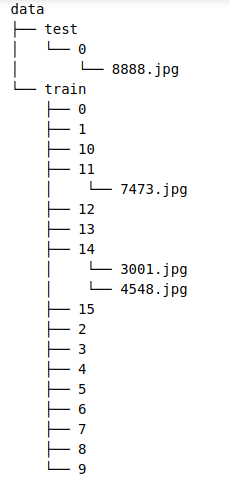
\includegraphics[width=80px]{img/directories.png}
    \caption{Organización de directorios para Pytorch}
    \label{directories}
  \end{subfigure}
 \begin{subfigure}{.6\textwidth}
   \centering
    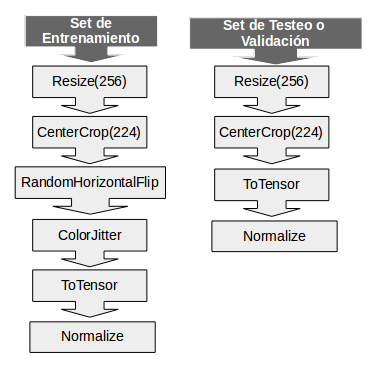
\includegraphics[width=150px]{img/transformaciones.png}
    \caption{ Pipeline de transformaciones  }
  \end{subfigure}
\end{figure}


Justificación: 

\begin{itemize}
  \item Resize(256) $\rightarrow$ CenterCrop(224): Dado que el modelo va a usar Transfer Learning sobre modelos entrenados con tamaños de entrada 224x224x3, las imagenes son redimensionadas a 256x256x3 para luego, mediante CenterCrop, ignorar los bordes quedándo con el centro, donde podría estar la información más relevante. 
  \item ToTensor: Transforma los bits en un tensor
  \item Normalize: Normaliza los datos para mejorar la convergencia  
\end{itemize}

Para el dataset de entrenamiento, además se incluyeron las siguientes transformaciones:

\begin{itemize}
  \item RandomHorizontalFlip: Debido al tipo de problema, una habitación vista de derecha a izquierda, o de izquierda a derecha pertenece a una misma categoría. Por ejemplo, una silla apuntando hacia la izquierda o la derecha no cambia la detección y poder invertir las imagenes permite darle mayor información al clasificador. 
  \item ColorJitter: Aplica cambios aletorios al brillo, constranste y saturación de la imagen. La idea es despegar un poco de los colores que se ven en la habitación. 
\end{itemize}

Otras transformaciones consideradas y descartadas: 

\begin{itemize}
  \item Grayscale: se probó convertir grayscale sin grandes resultados aparentemente porque los modelos pre-entrados usados trabajan con entradas a color. 
  \item RandomRotation: Dado que las habitaciones parten de un piso, rotarlas carece de sentido. Se probó con una pequeña rotación de 10 grados sin grandes cambios.
\end{itemize}

\subsection{Etiquetas y desbalanceo del conjunto de entrenamiento}

El conjunto de entrenamiento suministrado está desbalanceado, es decir, algunas categorías tienen demasiadas imágenes en comparación a otras. 

No modifiqué los datos ni excluí imágenes por esto. Simplemente, calculé los diferentes pesos de las categorías de las siguiente forma para ser usados por la función de pérdida (que va a ser un weighted categorical crossentropy, más información en las siguientes secciones).
 

\section{Modelado}
\label{sec:headings}

\subsection{Transferencia del aprendizaje - Transfer Learning}

En lugar de construir un modelo desde el llano, se optó por re-entrenar un modelo existente, cuyo pesos fueron calculados el dataset Imagenet.

Se elije este enforque porque estos modelos se encuentran hiper optimizados y entrenados durante días sobre los datos. Lograr algo similar requeriría mucho tiempo y esfuerzo que carecería de sentido en este contexto. 

Estos modelos son, además, un buen benchmark para evaluar cualquier modelo que se quiera diseñar desde cero. 
\begin{figure}[H]
\centering
    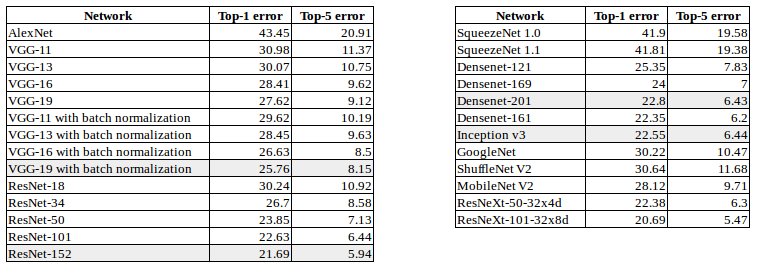
\includegraphics[width=400px]{img/pytorch-benchmark.png}
    \caption{Modelos pre-entrenados - Benchmark - Fuente: Pytorch}
    \label{models_bench}
\end{figure}
Para la competencia, se probaron modelos simples de pocas capas, intermedios y con muchas capas. Se probó con VGG19 con BatchNormalization, Resnet18, AlexNet, Resnet50 y Resnet101. Sin embargo, aquellos que tienen más capas son los que mejores resultados tuvieron: \textbf{Resnet152} y \textbf{Denset201}. 

Adicionalmente, se probó el modelo \textit{inception} que utiliza entradas de 299x299x3. Los resultados no fueron superiores que los dos detallados anteriormente.

La elección del modelo final tuvo dos etapas. La primera relacionada con evaluar distintos modelos con diferentes learning rates, optimizadores y parámetroes, y una segunda etapa, focalizada en la optimización de los modelos de interés.
 
En un comienzo, no todos los entrenamientos fueron bajo las mismas condiciones, hasta que se encontraron parámetros y modelos interesantes que fueron expuestos a fine tuning que detallo en la próxima sección.

Los resultados acompañan la lógica de que modelos más profundos captan mejor los detalles de los datos pero tienden a overfittear y ese fue el principal problema que apareció durante el entrenamiento. Además, la elección de Resnet152 y Densenet201 como candidatos está también justificada por los benchmarks presentados en la figura \ref{models_bench}.

Por falta de tiempo, excluyo de la optimización a VGG19 con Batch Normalization e Inception, que me parecen bastante interesantes y que me hubiera gustado profundizar. 

\subsubsection{Bottleneck features vs. entrenamiento del modelo completo}

También se consideró usar los modelos como features extractors, es decir, usar los pesos sobre los datos de entrenamiento y entrenar un modelo más pequeño que utilize esta información de entrada, pero los resultados no fueron tan buenos como reentrenar el modelo completo.\\

La técnica de reentrenar el modelo consiste en usar los pesos pre-calculados como pesos iniciales y reentrenar el modelo completo, no únicamente las capas finales. Este segundo aproach tuvo resultados superiores.

\subsection{El modelo}

El modelo que mejor funcionó fue un Resnet152. Las redes neuronales residuales proponen una solución al desvanecimiento del gradiente durante el entrenamiento. Esta compuesta por bloques residuales que poseen ademas un enlace que lleva al final del bloque aplicando la función identidad sobre la entrada. 

\begin{figure}[H]

  \begin{subfigure}{.4\textwidth}
  \begin{center}
    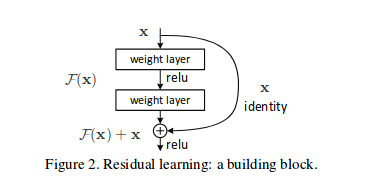
\includegraphics[width=\linewidth]{img/resnet_connection.png}
    \caption{Bloque Resnet}
    %\label{conn} 
  \end{center}
\end{subfigure}
\begin{subfigure}{.6\textwidth}
  \begin{center}
    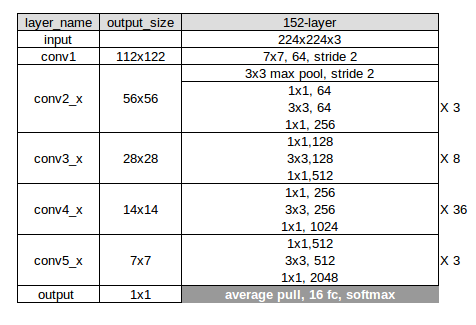
\includegraphics[width=200px]{img/network.png}
    \caption{Resnet-152 modificada . Salida 16 nodos. }
 \end{center}
\end{subfigure}
%\caption{Bloque Resnet}
\end{figure}

La última capa de esta red la he reemplazado por una capa completamente conectada que retorna 16 salidas, cada una correspondiente a la probabilidad de cada categoría. 


\subsection{Función de pérdida}

La elección de la función de pérdida (loss function) se vió relacionada con el tipo de problema a resolver. Dado que se trata de una clasificación elegí, en primer lugar, la función \textit{Categorical Crossentropy}. 

Los resultados no eran los esperados de manera equitativa en todas las categorías por la naturaleza de los datos, no se poseía una cantidad equilibrada de imágenes por categoría. Por lo tanto, decidí finalmente utlizar una variante que además considera los pesos, \textit{Weighted Categorical Crossentropy}.

Los pesos fueron calculados de la siguiente forma:

Dado $l_{i}$ con $0 \leq i \leq 15$ indicando cada una de las etiquetas:
\begin{center}
$ weight(l_{i}) = count(l_{max\_j}) / count(l_{i})$
\end{center}
siendo $0 \leq max\_j \leq 15$ y $max\_j$ id de la categoría con máxima cantidad de imágenes.

Estos pesos calculados, son pasados a la función de pérdida  \textit{Weighted Categorical Crossentropy} que los usa en el cálculo de la pérdida.

\begin{figure}[H]
  \begin{subfigure}{.5\textwidth}
  \begin{center}
    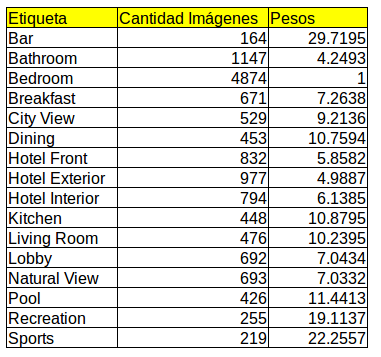
\includegraphics[width=150px]{img/weights.png}
    \caption{Pesos por categoria para todo el dataset }
  \end{center}
    \end{subfigure}
      \begin{subfigure}{.5\textwidth}
  \begin{center}
    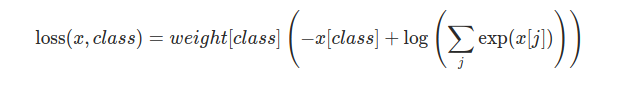
\includegraphics[width=250px]{img/CrossEntropyLoss.png}
    \caption{ Cálculo del Cross Entropy Loss usando pesos por Pytorch }
  \end{center}
        \end{subfigure}
\end{figure}

\section{Evaluación de los Resultados}
\label{sec:others}

\subsection{Optimización}

En la primer etapa de optimización busqué el modelo, optimizadores y parámetros que mejor resultados daban. Las mediciones que usé, en esta primer etapa, fueron los ploteos de accuracy y evolución de la función de pérdida, en validación y testeo. 

Como detallé anteriormente, los mejores resultados los obtuve con las siguiente combinaciones (en negrita): 

\begin{figure}[H]
  \centering
    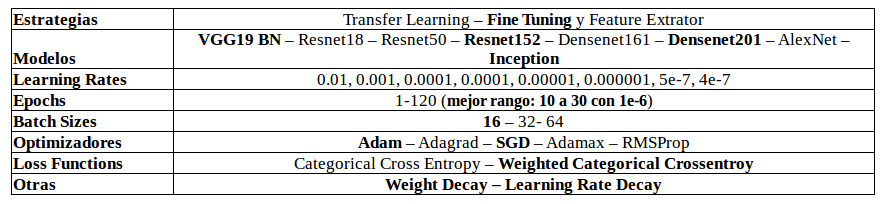
\includegraphics[width=300px]{img/tested.png}
    \caption{Combinaciones y modelos testeados. En negrita, las combinaciones que tuvieron mejores resultados}
    \label{models_bench2}
\end{figure}

Luego de la primer etapa de optimización, de la cual extraje dos modelos candidatos: Resnet153 y Densenet201, y algunos parámetros (batch\_size = 16, learning\_rate=1e-6 aprox.), realizé varios entrenamientos que me permitan encontrar el mejor optimizador.

El problema principal que tenía es que el entrenamiento tenía un techo del 80\% de accuracy sobre el conjunto de validación. Así también la función de pérdida planchaba cuando el learning rate era constante y tendía a overfitear.

\begin{figure}[H]
  \begin{subfigure}{.5\textwidth}
    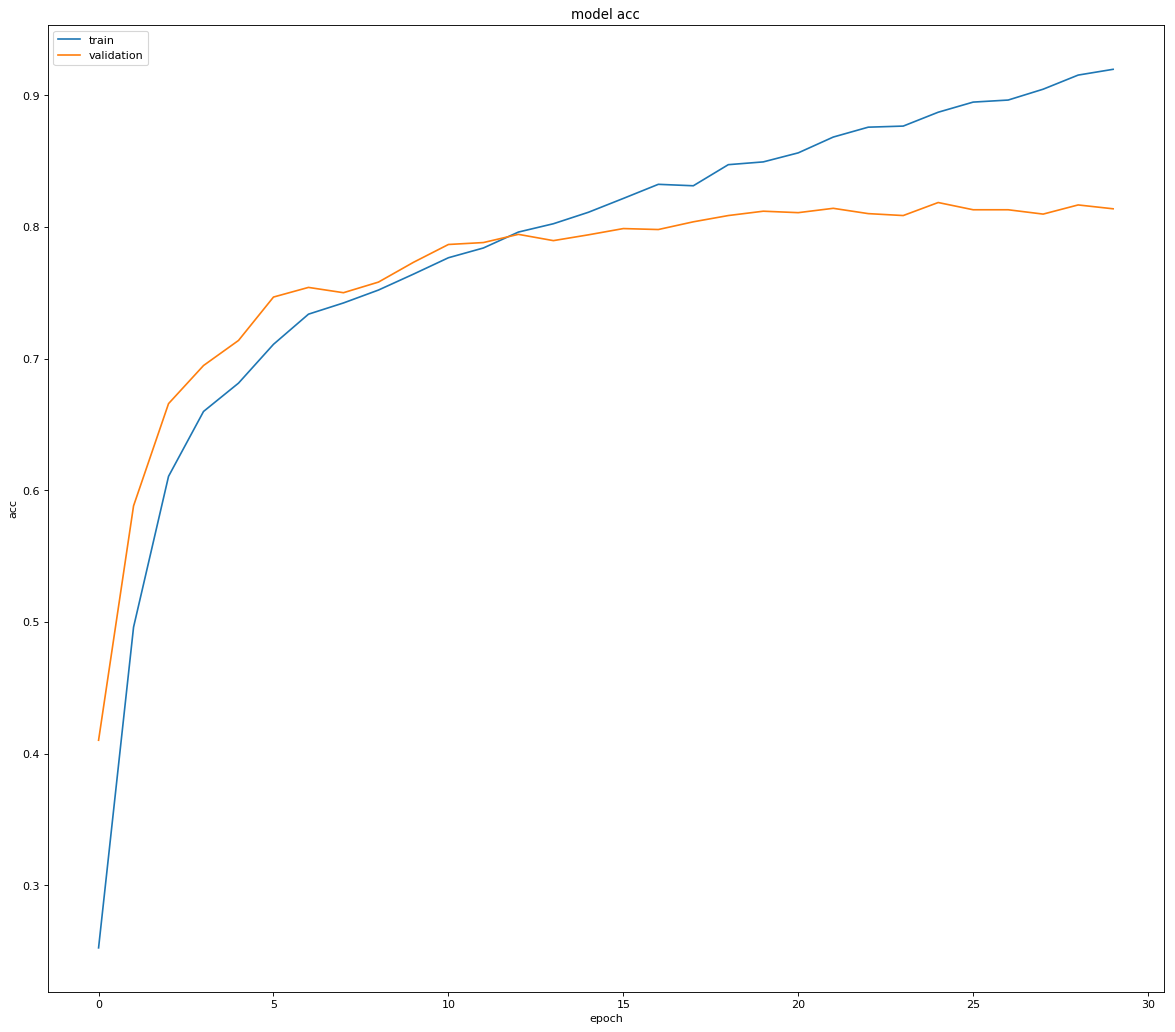
\includegraphics[width=\linewidth]{img/resnet152_Adam-1e-06-30ep16bs_1562750880-WEIGHTED-ACC.png}
    \caption{Accuracy}
    \label{adam_acc}
    \end{subfigure}
     \begin{subfigure}{.5\textwidth}
     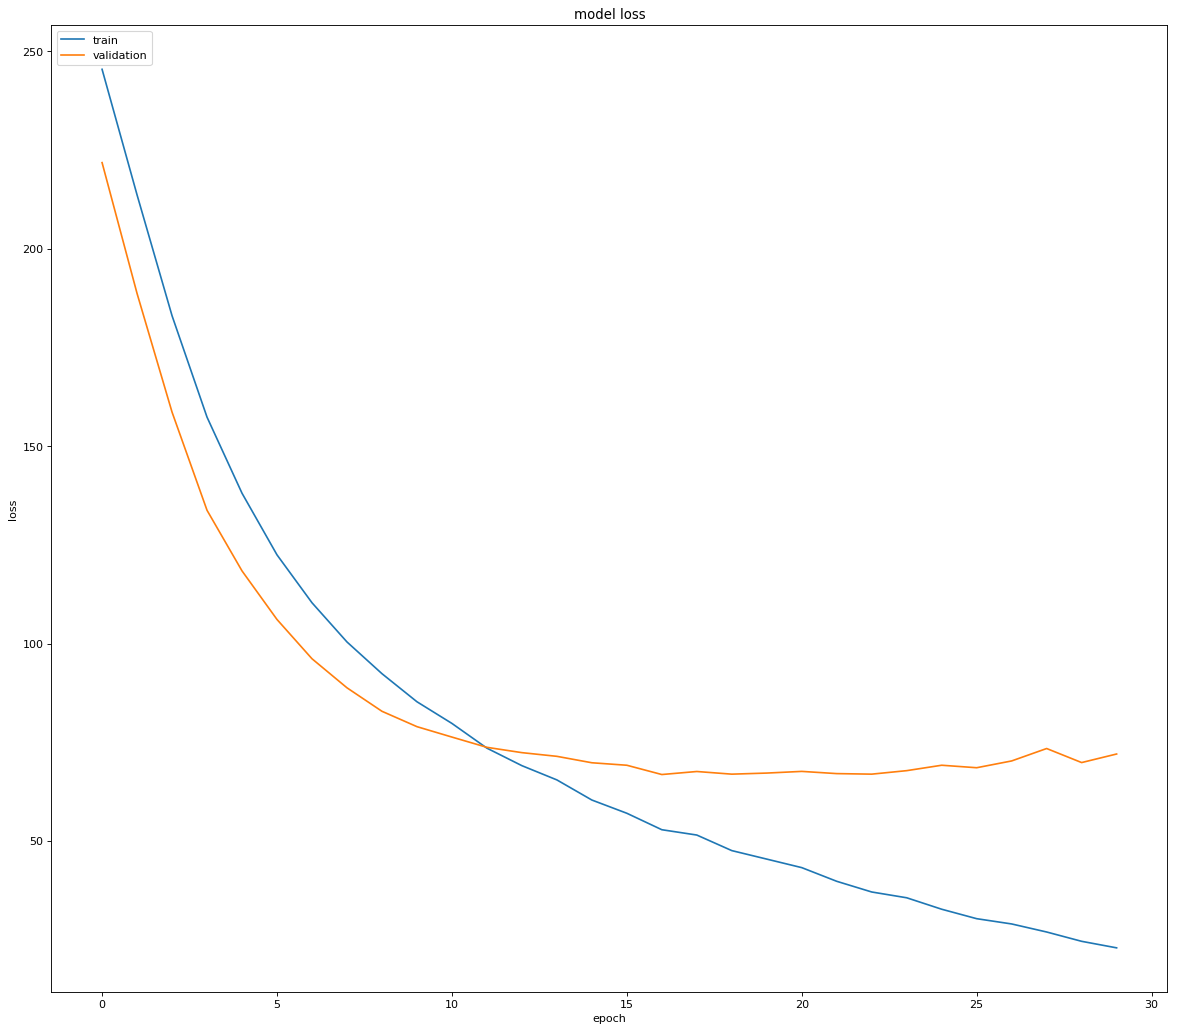
\includegraphics[width=\linewidth]{img/resnet152_Adam-1e-06-30ep16bs_1562750880-WEIGHTED.png}
   \caption{Loss Plot}
    \label{adam_loss}
    \end{subfigure}
\caption{Resnet152 LR: 1e-06 30 epochs }

\end{figure}

Por lo cual, la segunda etapa, la dediqué a usar técnicas de regularización L2 como \textbf{Weight Decay} y la modificación dinámica del learning rate, \textbf{Learning Rate Decay}. Pytorch trae la posibilidad de usar diferentes Schedulers con SGD que ante determinados eventos o con diferentes técnicas reducen el Learning Rate. En particular, seleccioné probar: \textbf{Cosine} y \textbf{ReduceLROnPlateau} con diferentes parámetros, como se observa a continuación:

\begin{figure}[H]
    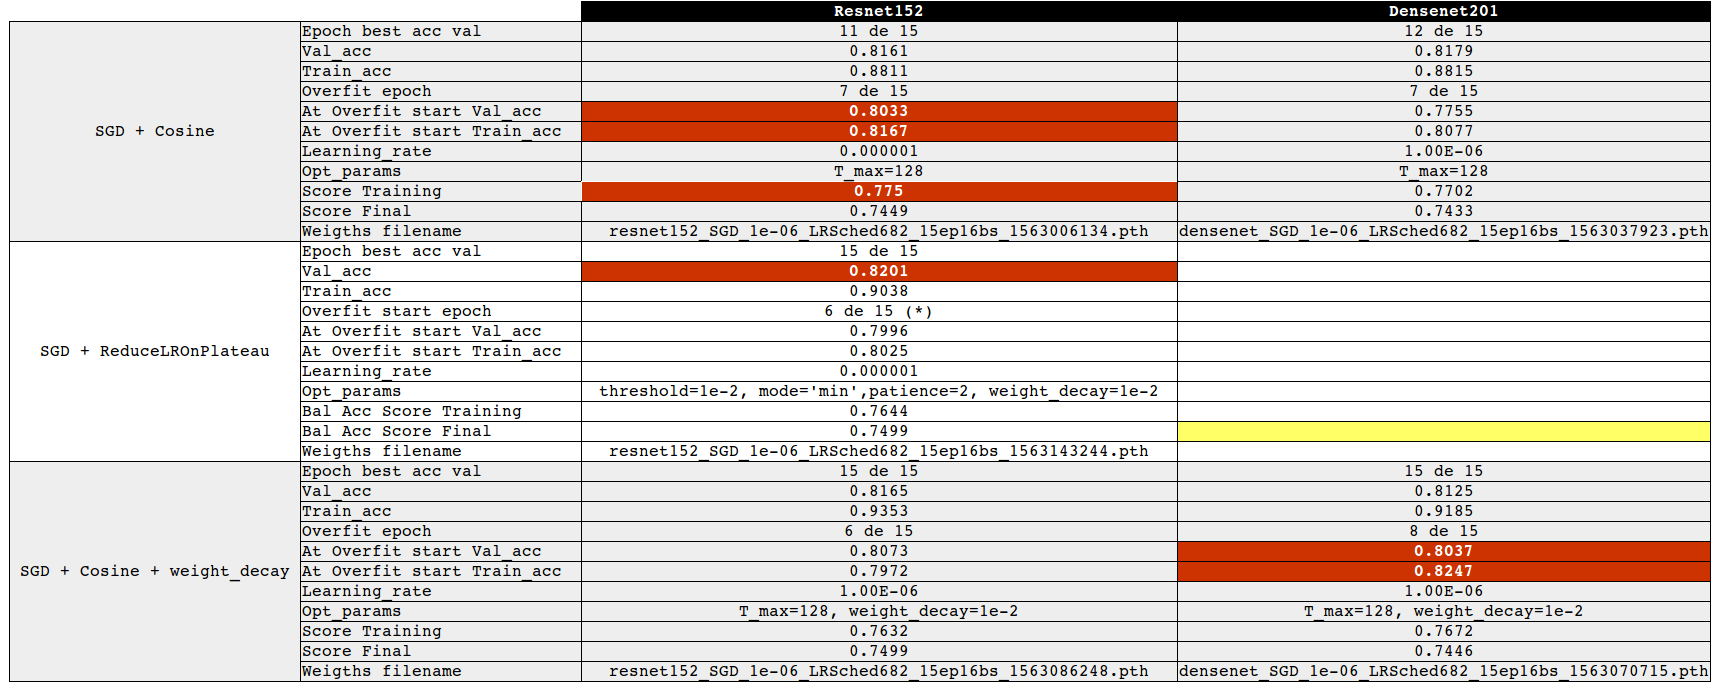
\includegraphics[width=\linewidth]{img/optim1.png}
\end{figure}

Si bien Cosine tenia buen Balanced Accuracy Score sobre el dataset de entrenamiento, la realidad, es que ReduceLROnPlateu parecía lograr mayor accuracy en validación a similar Balanced Accuracy Score en entrenamiento. La métrica del accuracy sobre validación era más importante dado que el Balanced Accuracy calculado dependia de la distribución actual del entrenamiento y desconocía como sería la distribución del dataset de la segunda etapa. Por lo cual, decidí que ReduceLROnPlateu con Resnet152 era la mejor combinación sobre la cual profundizar.

Vale aclarar que usar ReduceLROnPlateu, como dice su nombre, va reduciendo el learning rate a medida que transcurre el entrenamiento observando alguna métrica que uno puede indicar. En particular, elegí observar el loss en validación. Cuando se llegaba a un estancamiento, el scheduler lo reducía automáticamente. La idea era evitar el planchado mostrado en los gráficos anteriores. Incluso se puede elegir ser más agresivo con la reducción, pero por cuestiones de tiempo, no pude experimentar mucho con ese parámetro.

Así la siguiente optimización estuvo dada por el siguiente cuadro:

\begin{figure}[H]
    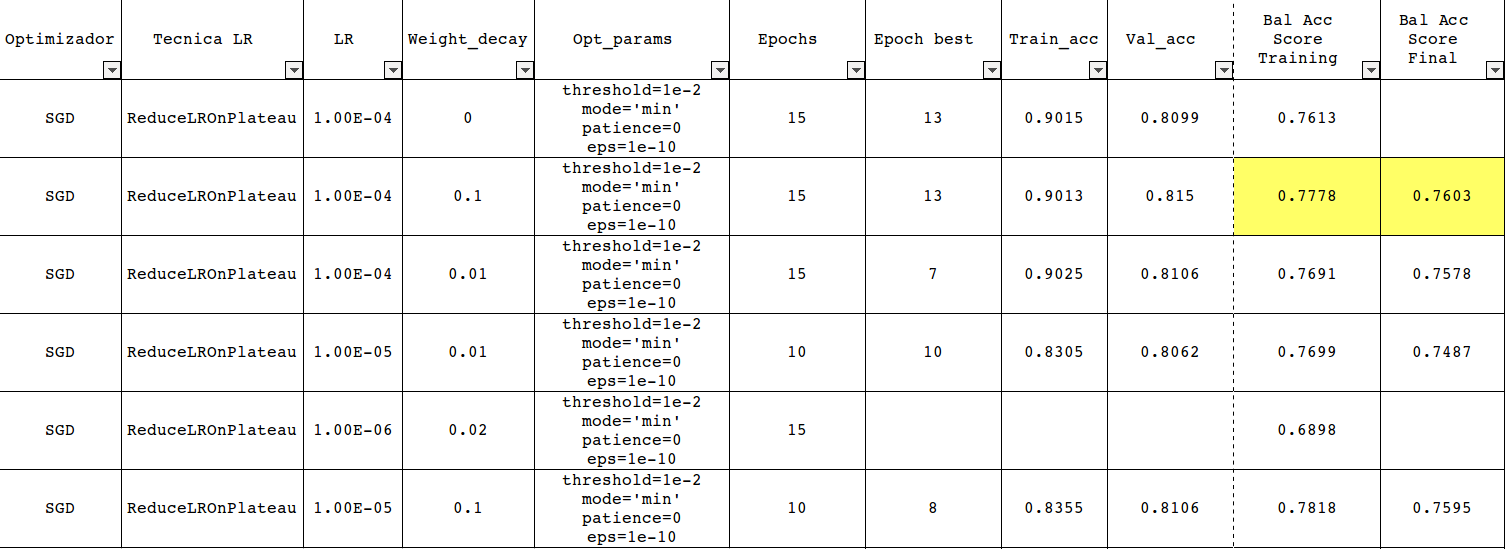
\includegraphics[width=\linewidth]{img/optim2.png}
\end{figure}

El indicado como test1 es la combinación que pasó a la segunda etapa. Lamentablemente, no llegué a subir la combinación test6 que se veía más balanceada en accuracy (overfiteaba menos) logrando casi los mismos scores.

\subsection{Visualización de los datos y las soluciones}

La solución final estaría dada por el modelo, función de pérdida, optimizador y parámetros:


\begin{scriptsize}

\textbf{Modelo}: Resnet152 + FC 16 softmax (Transfer Learning - Fine Tuning/Reentrenar con pesos)\\
\textbf{Función de Pérdida}: Weighted Categorical Crossentropy (torch.nn.CrossEntropyLoss weight=weights)\\
\textbf{Optimizador}: SGD (learning\_rate = 1e-4, weight\_decay=0.1) \\
\textbf{SGD Scheduler}: ReduceLROnPlateu (threshold=1e-2 mode='min',patience=0,eps=1e-10) sobre el loss en validación\\
\textbf{Batch Size}: 16\\
\textbf{Epochs}: 13 
\end{scriptsize}
\begin{figure}[H]
\centering
    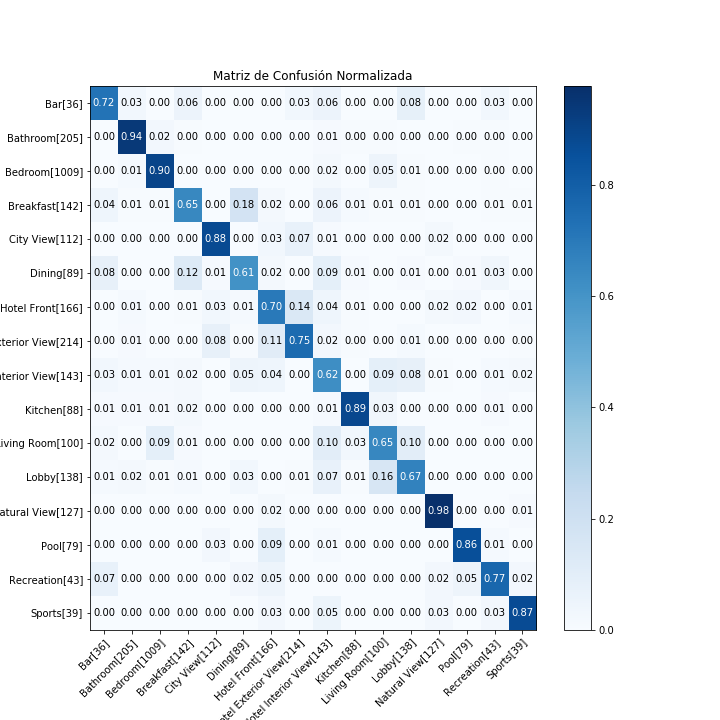
\includegraphics[width=350px]{img/confmat.png}
\end{figure}

Se deduce que por ejemplo, confunde el 18\% de los Breakfast con Dinning, lo cual suena lógico dado que ambos espacios se usan para comer y por ejemplo, pueden contar con mesas y sillas. \\
Luego, confunde un 16\% los Living Room con Lobby, similar razonamiento, ambos podrían incluir sillones. 


\begin{figure}[H]
  \begin{subfigure}{.5\textwidth}
    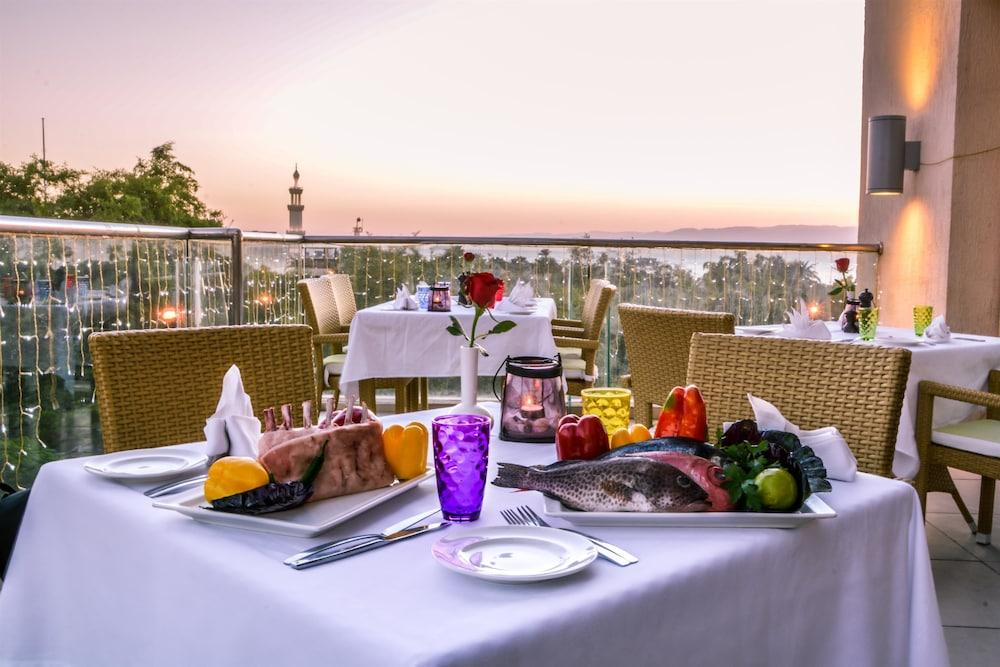
\includegraphics[width=\linewidth]{img/dinning.jpg}
    \caption{Dinning}
    \end{subfigure}
     \begin{subfigure}{.5\textwidth}
     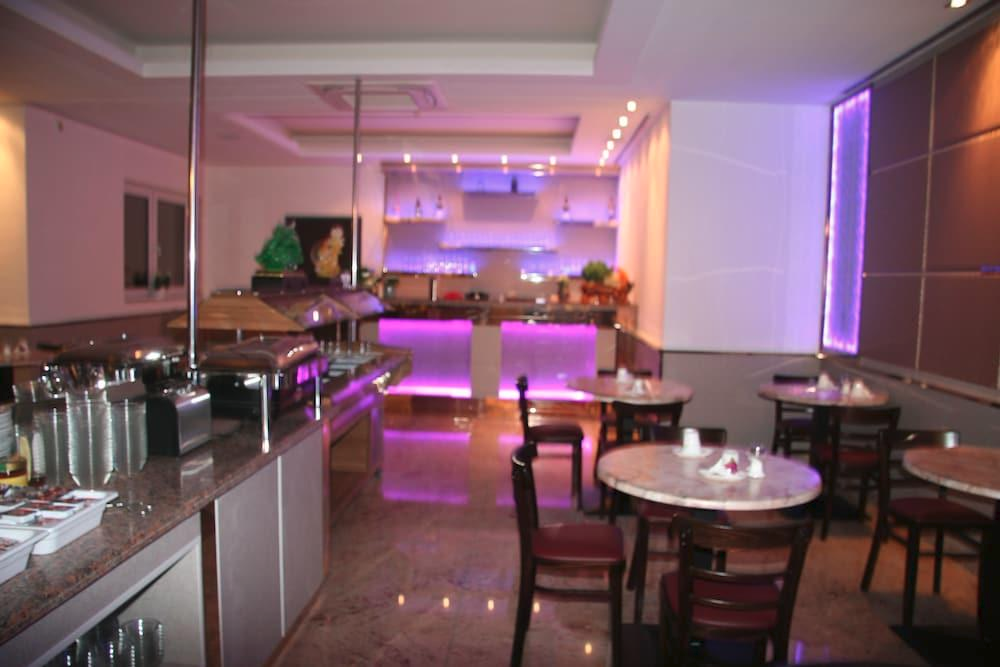
\includegraphics[width=\linewidth]{img/breakfast.png}
   \caption{Breakfast}
    \end{subfigure}
\caption{Errores de clasificación}
\label{fig:test}
\end{figure}

% \cite{kour2014real,kour2014fast} and see \cite{hadash2018estimate}.



% \bibliographystyle{unsrt}  
% %\bibliography{references}  %%% Remove comment to use the external .bib file (using bibtex).
% %%% and comment out the ``thebibliography'' section.
% %%% Comment out this section when you \bibliography{references} is enabled.
% \begin{thebibliography}{1}
%
% \bibitem{kour2014real}
% George Kour and Raid Saabne.
% \newblock Real-time segmentation of on-line handwritten arabic script.
% \newblock In {\em Frontiers in Handwriting Recognition (ICFHR), 2014 14th
%   International Conference on}, pages 417--422. IEEE, 2014.
%
% \bibitem{kour2014fast}
% George Kour and Raid Saabne.
% \newblock Fast classification of handwritten on-line arabic characters.
% \newblock In {\em Soft Computing and Pattern Recognition (SoCPaR), 2014 6th
%   International Conference of}, pages 312--318. IEEE, 2014.
%
% \bibitem{hadash2018estimate}
% Guy Hadash, Einat Kermany, Boaz Carmeli, Ofer Lavi, George Kour, and Alon
%   Jacovi.
% \newblock Estimate and replace: A novel approach to integrating deep neural
%   networks with existing applications.
% \newblock {\em arXiv preprint arXiv:1804.09028}, 2018.
%
% \end{thebibliography}
%

\end{document}
